\chapter{实验设计与结果分析}
\label{cha:experiments}

本章围绕所提双层 MARL 框架是否能够在多 UAV MEC 场景中改善系统级综合性能展开实验验证。实验首先给出仿真环境、对比方法和评估指标，然后从主实验、上层轨迹贡献、空间轨迹、卸载分布、下层消融、端到端 baseline 以及 DSR-priority 配置等角度分析方法的有效性与边界。核心结论是：完整双层方法显著降低 UAV 侧能耗、提升服务公平性并消除低电量离线用户，但在能耗优先配置下会牺牲部分 deadline satisfaction rate（DSR）；通过调整奖励权重和 Lagrange 约束目标，可以部分恢复 DSR。

\section{仿真环境与参数}
\label{sec:simulation-setup}

实验区域为 $700$m $\times$ 700m，系统包含 $N=5$ 架 UAV、$M=100$ 个 UE 和 $1$ 个 MBS。每个 episode 包含 $T=1000$ 个 time slots，每个 time slot 时长为 $\tau = 1$s。UAV 飞行高度 $H=100$m，最大速度 $v_{max}=15$m/s，覆盖半径 $R_c=100$m，感知范围 $460$m，最小 UAV 间距 $200$m。系统包含 25 类服务和 50 类内容文件，服务 deadline 在 $[0.65, 2.10]$s 范围内生成。MBS 固定算力 $f_{mbs} = 200 \times 10^9$ cycles/s。UAV 计算能力在 $[40, 90] \times 10^9$ cycles/s 之间随机生成。

UE 电池容量 $B_{max}=500$J，临界阈值 $B_{low}=50$J，待机功耗 $P_{static}=0.01$W。飞行功率 $P_{move}=300$W，悬停功率 $P_{hover}=150$W。WPT 发射功率 $P_{wpt}=50$W，采集增益 $G=5\times10^5$，采集效率 $\eta=0.8$。

所有 MARL 策略使用 PyTorch 实现，MAPPO 采用 2 层 MLP（hidden dim=128），attention 模块隐层维度为 64（ATTN\_HIDDEN\_DIM=64），Adam 优化器，learning rate$=3\times10^{-4}$，PPO clip $\epsilon=0.2$，discount $\gamma=0.99$，GAE $\lambda=0.95$。

正式实验采用 3 个 training seeds（42, 84, 126）和 10 个 workload seeds（42-420），每个 workload seed 运行 6 个 episodes。统计单元为 (training seed, workload seed) 的 episode mean，每个策略共有 $N=30$ 个统计样本。本文报告 mean、std、95\% CI、paired delta、paired t-test 和 Wilcoxon 检验。

\section{对比方法}
\label{sec:comparison-methods}

\subsection{主实验策略组合}

主实验比较五组策略组合，如表 \ref{tab:main-strategies} 所示。

\begin{table}[!htbp]
    \centering
    \bicaption{主实验策略组合}{Main experiment strategy combinations}
    \label{tab:main-strategies}
    \begin{tabular}{|l|c|c|c|}
        \hline
        组合方案 & 轨迹控制 & 卸载策略 & 角色 \\
        \hline
        uncoordinated\_greedy\_\_heuristic & uncoordinated greedy & heuristic & 基础参考 \\
        attention\_mappo\_\_heuristic & attention-MAPPO & heuristic & 上层贡献 \\
        uncoordinated\_greedy\_\_lower\_mappo & uncoordinated greedy & lower MAPPO & 下层贡献 \\
        attention\_mappo\_\_lower\_mappo & attention-MAPPO & lower MAPPO & 分别训练后组合 \\
        full\_hierarchical\_marl & attention-MAPPO & lower MAPPO & 完整双层联合训练 \\
        \hline
    \end{tabular}
\end{table}

\subsection{下层消融实验}

下层消融实验以 \texttt{lower\_full}（即 \texttt{attention\_mappo\_\_lower\_mappo}）为参考，如表 \ref{tab:ablation-strategies} 所示。

\begin{table}[!htbp]
    \centering
    \bicaption{下层消融实验配置}{Lower-layer ablation configurations}
    \label{tab:ablation-strategies}
    \begin{tabular}{|l|c|c|c|}
        \hline
        消融方法 & Attention & Quality mask & Lagrange \\
        \hline
        lower\_full & yes & yes & yes \\
        lower\_no\_mask & yes & no & yes \\
        lower\_no\_lagrange & yes & yes & no \\
        lower\_no\_attention & no & yes & yes \\
        \hline
    \end{tabular}
\end{table}

\subsection{额外 baseline}

为进一步界定 attention 机制和双层分解的适用边界，本文还补充报告上层 \texttt{vanilla\_mappo\_\_heuristic} 消融、attention 权重可视化和 \texttt{joint\_end\_to\_end\_mappo} 端到端联合 MAPPO baseline。在此基础上，本文进一步构建扩展 baseline 矩阵，将 \texttt{random}、\texttt{uniform}、\texttt{ippo}、\texttt{vanilla\_mappo}、\texttt{joint\_mappo} 和本文方法置于同一评估协议下比较。学习式方法采用 3 个 training seeds 和 10 个 workload seeds，统计单元为 (training seed, workload seed)，共 $N=30$；非学习式方法以 workload seed 为统计单元，共 $N=10$。该扩展矩阵用于验证本文方法相对经典随机、均匀、独立学习、普通 MAPPO 和端到端联合 MAPPO 的综合优势与边界。

\section{评估指标}
\label{sec:metrics}

本文使用以下评估指标：

\begin{itemize}
    \item \textbf{Reward ($R_t$)}：第 \ref{sec:optimization-objective} 节定义的系统级综合奖励
    \item \textbf{Latency ($L$)}：所有 UE 的总时延（含 $T_{penalty}=20$s 未服务惩罚）
    \item \textbf{Energy ($E$)}：UAV 侧总能耗（含飞行、悬停、计算、通信、WPT）
    \item \textbf{Fairness ($J$)}：基于各 UE 的 service\_coverage 计算 Jain 指数，衡量用户服务覆盖公平性
    \item \textbf{DSR}：deadline satisfaction rate，被服务且满足 deadline 的请求比例
    \item \textbf{offline\_rate ($O$)}：电池低于 $B_{low}$ 的 UE 比例
    \item \textbf{Offloading ratios}：local/cooperative/MBS 卸载比例。主实验表格沿用已处理请求作为分母；扩展 baseline 矩阵进一步报告 processed-denominator offloading ratios
    \item \textbf{MBS load ratio}：卸载至 MBS 的请求负载比例。为避免与 MBS offloading ratio 混淆，扩展 baseline 矩阵采用 generated-denominator MBS load ratio，即 MBS 请求数占全部生成服务请求数的比例
\end{itemize}

\section{主实验结果}
\label{sec:main-results}

表 \ref{tab:main-results} 汇总了主实验中各策略的均值和标准差（mean $\pm$ std）。该组实验检验双层分解的主张：上层轨迹学习主要改善空间部署与服务公平性，下层卸载学习主要改变能耗和卸载行为，完整联合训练应在二者之间形成更优折中。

\begin{table}[!htbp]
    \centering
    \bicaption{主实验结果（mean $\pm$ std, $N=30$）}{Main experiment results (mean $\pm$ std, $N=30$)}
    \label{tab:main-results}
    \resizebox{\textwidth}{!}{
    \begin{tabular}{l|rr|rr|rr|rr}
        \hline
        策略 & Reward & & Energy (M) & & DSR & & Fairness & \\
        \hline
        unco+heuristic & -5933.9 & $\pm$ 195.6 & 114.70 & $\pm$ 15.4 & 0.2734 & $\pm$ 0.029 & 0.7745 & $\pm$ 0.077 \\
        att+heuristic & \textbf{-2128.6} & $\pm$ 389.7 & 111.81 & $\pm$ 10.6 & \textbf{0.2879} & $\pm$ 0.032 & \textbf{0.9299} & $\pm$ 0.036 \\
        unco+lower & -5274.4 & $\pm$ 141.3 & 42.85 & $\pm$ 13.6 & 0.1891 & $\pm$ 0.029 & 0.7737 & $\pm$ 0.080 \\
        att+lower & \textbf{-1599.4} & $\pm$ 330.1 & 53.32 & $\pm$ 12.4 & 0.2170 & $\pm$ 0.035 & \textbf{0.9281} & $\pm$ 0.035 \\
        full\_hierarchical & \textbf{-1451.7} & $\pm$ 373.7 & 58.06 & $\pm$ 7.0 & 0.2083 & $\pm$ 0.019 & \textbf{0.9363} & $\pm$ 0.041 \\
        \hline
    \end{tabular}}
\end{table}

表 \ref{tab:main-results}（续）补充了 Offline\% 和卸载比例指标。

\begin{table}[!htbp]
    \centering
    \bicaption{主实验结果（续）}{Main experiment results (continued)}
    \label{tab:main-results-cont}
    \resizebox{\textwidth}{!}{
    \begin{tabular}{l|rr|rr|rr}
        \hline
        策略 & Offline\% & & Local\% & Coop\% & MBS load\% \\
        \hline
        unco+heuristic & 0.58\% & & 47.1\% & 50.1\% & 2.6\% \\
        att+heuristic & 0.10\% & & 47.2\% & 50.0\% & 2.7\% \\
        unco+lower & 0.53\% & & 52.6\% & 30.1\% & 17.1\% \\
        att+lower & 0.11\% & & 41.7\% & 44.6\% & 13.7\% \\
        full\_hierarchical & \textbf{0.00\%} & & 46.4\% & 42.4\% & 11.1\% \\
        \hline
    \end{tabular}}
\end{table}

表 \ref{tab:paired-comparison} 给出了 Full Hierarchical MARL 相对基础参考的配对比较。

\begin{table}[!htbp]
    \centering
    \bicaption{Full Hierarchical MARL 相对基础参考的配对比较}{Paired comparison of Full Hierarchical MARL vs baseline}
    \label{tab:paired-comparison}
    \begin{tabular}{l|c|c|c|c}
        \hline
        指标 & Mean Delta & 95\% CI & paired t $p$ & Effect \\
        \hline
        Reward & \textbf{+4482.2} & [4338.3, 4626.1] & $1.0\times10^{-32}$ & $\uparrow$ \\
        Energy & \textbf{-56.64M} & [-61.97M, -51.31M] & $1.7\times10^{-19}$ & $\uparrow$ \\
        Fairness & \textbf{+0.1617} & [0.1305, 0.1929] & $1.7\times10^{-11}$ & $\uparrow$ \\
        DSR & -0.0651 & [-0.0779, -0.0524] & $2.4\times10^{-11}$ & $\downarrow$ \\
        offline\_rate & -0.0058 & [-0.0099, -0.0017] & 0.0067 & $\uparrow$ \\
        Coop ratio & -0.0776 & [-0.1005, -0.0546] & $1.3\times10^{-7}$ & $\downarrow$ \\
        MBS load ratio & +0.0387 & [0.0319, 0.0454] & $1.7\times10^{-12}$ & 增加 \\
        \hline
    \end{tabular}
\end{table}

完整双层 MARL 的主要收益集中在系统奖励、能耗、公平性和在线率四个维度。相对基础参考，reward 提升 4482.2（$p = 1.0\times10^{-32}$），UAV 侧能耗降低 56.64M（$p = 1.7\times10^{-19}$），公平性提升 0.162（$p = 1.7\times10^{-11}$），offline rate 降至 0.00\%。这一结果说明，双层框架能够通过轨迹协同和请求级卸载重分配降低高能耗服务模式，并使服务覆盖在 UE 间更加均衡。需要同时指出的是，DSR 是该配置下的明确负向结果：完整方法的 DSR 从 0.2734 降至 0.2083（$\Delta=-0.0651$, $p=2.4\times10^{-11}$）。因此，能耗优先主配置证明的是能耗、公平性和在线率收益，而不是 DSR 最优。

\begin{figure}[!htbp]
    \centering
    
\includegraphics[width=0.92\textwidth]{docs/figures/图5-7_主实验多指标对比.pdf}
    \bicaption{主实验多指标对比}{Main experiment multi-metric comparison}
    \label{fig:main-comparison}
\end{figure}

\section{上层贡献分析}
\label{sec:upper-contribution}

仅替换上层轨迹策略（\texttt{att+heuristic} vs \texttt{uncoordinated\_greedy\_\_heuristic}），在保持 heuristic 卸载不变的情况下：
\begin{itemize}
    \item Reward：-5933.9 $\rightarrow$ -2128.6（$\Delta=+3805.4$, $p=3.0\times10^{-30}$）
    \item Fairness：0.7745 $\rightarrow$ 0.9299（$\Delta=+0.1554$, $p=3.4\times10^{-10}$）
    \item Energy：114.70M $\rightarrow$ 111.81M（$\Delta=-2.89M$, $p=0.086$）
    \item DSR：0.2734 $\rightarrow$ 0.2879（$\Delta=+0.0145$, $p=0.084$）
\end{itemize}

该对比表明，上层 attention-MAPPO 的主要贡献不是直接降低能耗，而是通过协同轨迹控制改善空间服务均衡性。Reward 和 fairness 的提升达到统计显著，energy 和 DSR 仅呈改善趋势且未达到显著水平，因此上层模块更适合解释为公平性和空间部署模块，而不是独立的服务质量优化模块。

\textbf{补充表 A. 上层 vanilla MAPPO 消融（training seed=42, 4 workload seeds $\times$ 8 episodes）}

\begin{table}[!htbp]
    \centering
    \bicaption{上层 vanilla MAPPO 消融结果}{Upper-layer vanilla MAPPO ablation results}
    \label{tab:vanilla-ablation}
    \resizebox{\textwidth}{!}{
    \begin{tabular}{l|rr|rr|rr|rr}
        \hline
        策略 & Reward & & Latency & & Energy (M) & & DSR & \\
        \hline
        vanilla\_mappo\_\_heuristic & \textbf{-1462.6} & $\pm$ 328.7 & \textbf{841994} & $\pm$ 95239 & 120.11 & $\pm$ 15.69 & \textbf{0.2822} & $\pm$ 0.0278 \\
        attention\_mappo\_\_heuristic & -2222.1 & $\pm$ 890.6 & 1135453 & $\pm$ 132493 & \textbf{114.55} & $\pm$ 13.26 & 0.2799 & $\pm$ 0.0317 \\
        \hline
    \end{tabular}}
\end{table}

在该补充实验中，vanilla\_mappo 在 reward、latency 和 fairness 上优于 attention\_mappo；attention 相对 vanilla 的 latency 增加约 293458（paired t-test $p=0.0085$），reward 降低约 759.5（$p=0.0889$）。另一方面，attention-MAPPO 的 energy 更低（约 -5.57M，$p=0.102$），offline rate 更低，MBS load ratio 也显著更低（0.99\% vs 1.41\%，$p=0.0155$）。

\section{轨迹可视化分析}
\label{sec:trajectory-visualization}

由于本文方法同时包含上层轨迹控制和下层请求级卸载决策，仅依赖表格指标难以直观展示不同策略在空间维度上的行为差异。考虑到评估过程中 UE 位置和请求状态会随时间变化，单一时刻的用户散点不能完整代表整个 episode 的服务需求分布。因此，图 \ref{fig:trajectory-user-distribution} 仅展示同一评估场景下不同算法的无人机二维飞行轨迹，用于分析策略在空间移动模式和移动代价上的差异。该图基于 training seed 42 和 workload seed 42 的第一个评估 episode 绘制。其中，彩色曲线表示 5 架无人机在整个评估 episode 中的水平飞行轨迹，空心圆表示无人机起点，实心方块表示终点，箭头表示移动方向，黑色五角星表示宏基站位置。各子图左下角进一步给出了该 episode 内 5 架无人机的累计飞行距离。

\begin{figure}[!htbp]
    \centering
    \begin{minipage}{0.48\textwidth}
        \centering
        
\includegraphics[width=\linewidth]{docs/figures/图5-6a_随机策略无人机二维轨迹.pdf}
        \\(a) 随机策略
    \end{minipage}
    \hfill
    \begin{minipage}{0.48\textwidth}
        \centering
        
\includegraphics[width=\linewidth]{docs/figures/图5-6b_IPPO无人机二维轨迹.pdf}
        \\(b) IPPO
    \end{minipage}

    \vspace{0.8em}

    \begin{minipage}{0.48\textwidth}
        \centering
        
\includegraphics[width=\linewidth]{docs/figures/图5-6c_VanillaMAPPO无人机二维轨迹.pdf}
        \\(c) Vanilla MAPPO
    \end{minipage}
    \hfill
    \begin{minipage}{0.48\textwidth}
        \centering
        
\includegraphics[width=\linewidth]{docs/figures/图5-6d_本文方法无人机二维轨迹.pdf}
        \\(d) 本文方法
    \end{minipage}
    \bicaption{不同算法下无人机二维飞行轨迹对比}{Comparison of two-dimensional UAV trajectories under different algorithms}
    \label{fig:trajectory-user-distribution}
\end{figure}

从图 \ref{fig:trajectory-user-distribution} 可以看出，随机策略的移动方向缺乏稳定目标，轨迹更多体现为无规则探索，各 UAV 之间缺乏协调，累计飞行距离为 53.6 km。IPPO 和 Vanilla MAPPO 形成了较明显的局部移动模式，其中 IPPO 更倾向于快速靠近部分服务区域，因此在平均时延指标上表现较优，但两者的累计飞行距离分别达到 68.2 km 和 69.2 km，表明其降低时延的同时带来了较高移动代价。相比之下，本文方法的轨迹更加紧凑，累计飞行距离仅为 39.7 km，明显低于其他三种方法。该可视化结果并不直接证明本文方法在所有服务指标上最优，而是说明其上层轨迹策略在给定动态请求环境下能够减少不必要移动。结合表 \ref{tab:main-results} 以及后续卸载分布分析可知，本文方法的主要优势并不是轨迹形态或单一时延指标最优，而是在较低移动能耗、有效服务完成和协作卸载之间取得更有利的综合权衡。

\section{卸载分布分析}
\label{sec:offloading-analysis}

\begin{figure}[!htbp]
    \centering
    
\includegraphics[width=0.88\textwidth]{docs/figures/图5-8_卸载分布对比.pdf}
    \bicaption{卸载分布对比}{Offloading distribution comparison}
    \label{fig:offloading-dist}
\end{figure}

卸载分布的变化解释了能耗收益的来源。Heuristic 基线主要依赖 local 和 cooperative 两类执行方式，MBS load 仅为 2.6--2.7\%；引入下层 MAPPO 后，策略开始更主动地在 local、cooperative 和 MBS 之间分配请求，其中 MBS load 提升至 11--17\%。完整双层方法没有选择最激进的 MBS 使用方式，而是在 local 46.4\%、cooperative 42.4\%、MBS load 11.1\% 的分布下将 offline rate 降至 0.00\%。这说明下层策略的作用不是单纯增加某一种卸载模式，而是在能耗、可服务性和 MBS 约束之间重新分配请求。

\section{消融实验结果}
\label{sec:ablation-results}

表 \ref{tab:ablation-results} 给出了下层消融实验的详细结果。

\begin{table}[!htbp]
    \centering
    \bicaption{下层消融实验结果（相对于 lower\_full）}{Lower-layer ablation results (relative to lower\_full)}
    \label{tab:ablation-results}
    \begin{tabular}{l|rr|rr|rr}
        \hline
        消融 & Reward & & Energy (M) & & DSR & \\
        \hline
        lower\_full & -1599.4 & & 53.32 & & 0.2170 & \\
        no\_mask & -1556.3 & & 48.26 & & 0.1945 & \\
        no\_lagrange & -1585.9 & & 51.12 & & 0.1981 & \\
        no\_attention & -1626.7 & & 54.01 & & \textbf{0.2094} & \\
        \hline
    \end{tabular}
\end{table}

下层消融结果表明，三个组件分别约束不同类型的卸载行为。移除 quality mask 后，MBS load ratio 从 13.7\% 升至 18.0\%，reward 略有上升但未达到统计显著（+43.1, $p=0.09$），说明 mask 的作用主要是限制低质量或高风险 MBS 使用，而不是直接提高单一回合 reward。移除 Lagrange 约束的影响最明显：MBS load ratio 从 13.7\% 升至 25.0\%（$\Delta=+11.3$pp, $p=6.5\times10^{-5}$），表明该约束是抑制 MBS 依赖和维持负载边界的关键机制。移除 request attention 后，cooperative ratio 从 44.6\% 降至 34.4\%，local ratio 从 41.7\% 升至 48.2\%，而 DSR 与 lower\_full 接近（0.2094 vs 0.2170）。因此，attention 的主要作用是帮助策略识别可利用的协作卸载机会，而不是单独决定 DSR 水平。

\begin{figure}[!htbp]
    \centering
    
\includegraphics[width=0.92\textwidth]{docs/figures/图5-9_下层消融实验对比.pdf}
    \bicaption{消融实验对比}{Ablation experiment comparison}
    \label{fig:ablation-compare}
\end{figure}

\section{端到端 joint MAPPO baseline}
\label{sec:joint-mappo}

为回应"为什么不直接训练单一端到端策略同时输出轨迹和卸载动作"的问题，本文实现了 \texttt{joint\_mappo} baseline。该模型使用单一 MAPPO actor 同时输出 UAV 连续轨迹动作和请求级离散卸载动作，并使用联合观测与统一 PPO 更新，不复用已训练的上层或下层模型。

\textbf{补充表 B. 端到端 joint MAPPO 评估结果（training seed=42, 4 workload seeds $\times$ 8 episodes）}

\begin{table}[!htbp]
    \centering
    \bicaption{端到端 joint MAPPO 评估结果}{End-to-end joint MAPPO evaluation results}
    \label{tab:joint-mappo}
    \begin{tabular}{l|rr|rr|rr|rr}
        \hline
        策略 & Reward & & Latency & & Energy (M) & & DSR & \\
        \hline
        joint\_end\_to\_end\_mappo & -9865.1 & $\pm$ 325.6 & 1580604 & $\pm$ 267198 & 81.58 & $\pm$ 31.25 & 0.1349 & $\pm$ 0.0761 \\
        \hline
    \end{tabular}
\end{table}

端到端 joint MAPPO 在训练日志中能够获得一定的 recent reward，但独立 workload 评估结果明显退化：平均 reward 为 -9865.1，DSR 仅为 0.1349，fairness 为 0.4581，均显著弱于分层策略。该负向 baseline 支持本文的结构选择：在相同训练预算下，将连续轨迹控制和请求级离散卸载直接合并到单一 actor 会扩大联合动作空间，并加重 credit assignment 难度；双层分解虽然引入模块边界，但提高了样本效率、训练稳定性和行为可解释性。

\section{扩展 baseline 矩阵实验}
\label{sec:baseline-matrix-v2}

为避免仅依赖单一 baseline 或单一随机种子造成结论偏差，本文进一步补充扩展 baseline 矩阵实验。该实验包含六类方法：随机策略（Random）、均匀卸载策略（Uniform）、独立 PPO（IPPO）、普通 MAPPO（Vanilla MAPPO）、端到端联合 MAPPO（Joint MAPPO）以及本文方法（Proposed）。学习式方法均在 3 个 training seeds 下训练，并在 10 个 workload seeds 上评估；非学习式方法不涉及训练种子，因此以 10 个 workload seeds 作为统计单元。所有学习式方法的统计样本数为 $N=30$，非学习式方法为 $N=10$。比较时，学习式 baseline 与本文方法按 (training seed, workload seed) 配对，非学习式 baseline 则先对本文方法的 training seeds 取均值后按 workload seed 配对。

\begin{figure}[!htbp]
    \centering
    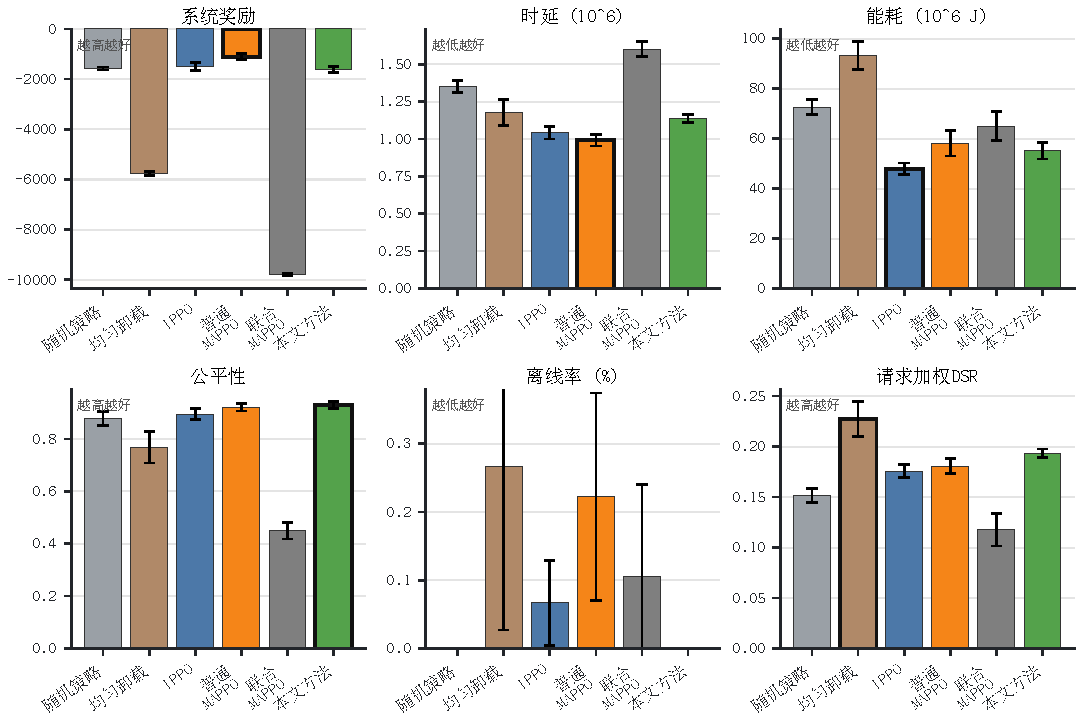
\includegraphics[width=0.96\textwidth]{docs/figures/图5-14_扩展baseline矩阵多指标对比.pdf}
    \bicaption{扩展 baseline 矩阵多指标对比}{Multi-metric comparison in the extended baseline matrix}
    \label{fig:baseline-matrix-overview}
\end{figure}

图 \ref{fig:baseline-matrix-overview} 表明，本文方法的优势主要集中在系统公平性、在线稳定性和请求级服务质量，而不是单一 latency 或 scalar reward 的全面最优。Proposed 的 final fairness 为 0.9290，在所有学习式方法中最高；相对 IPPO、Vanilla MAPPO 和 Joint MAPPO 分别提升约 3.84\%、0.96\% 和 107.14\%。同时，Proposed 的 final offline rate 和 step-mean offline rate 均为 0，显著低于 IPPO、Vanilla MAPPO、Joint MAPPO 和 Uniform，说明所提双层策略能够更稳定地避免低电量或服务失衡导致的离线现象。

在 deadline satisfaction 方面，Proposed 的 request-weighted DSR 为 0.1934，相比 IPPO、Vanilla MAPPO、Joint MAPPO 和 Random 分别提升约 10.09\%、7.03\%、64.53\% 和 27.71\%。但 Uniform 的 request-weighted DSR 为 0.2273，高于 Proposed。因此本文不将 DSR 描述为全局最优，而将其解释为：在学习式 baseline 和随机策略之间，本文方法获得了更高的请求加权截止期满足率；相对 Uniform，本文方法则以更低能耗、更高公平性和更低 MBS 负载换取部分 DSR。能耗方面，Proposed 相比 Vanilla MAPPO、Joint MAPPO、Random 和 Uniform 分别降低约 4.98\%、15.06\%、24.04\% 和 40.82\%，但高于 IPPO，说明本文方法的能耗优势同样具有明确边界。

\begin{figure}[!htbp]
    \centering
    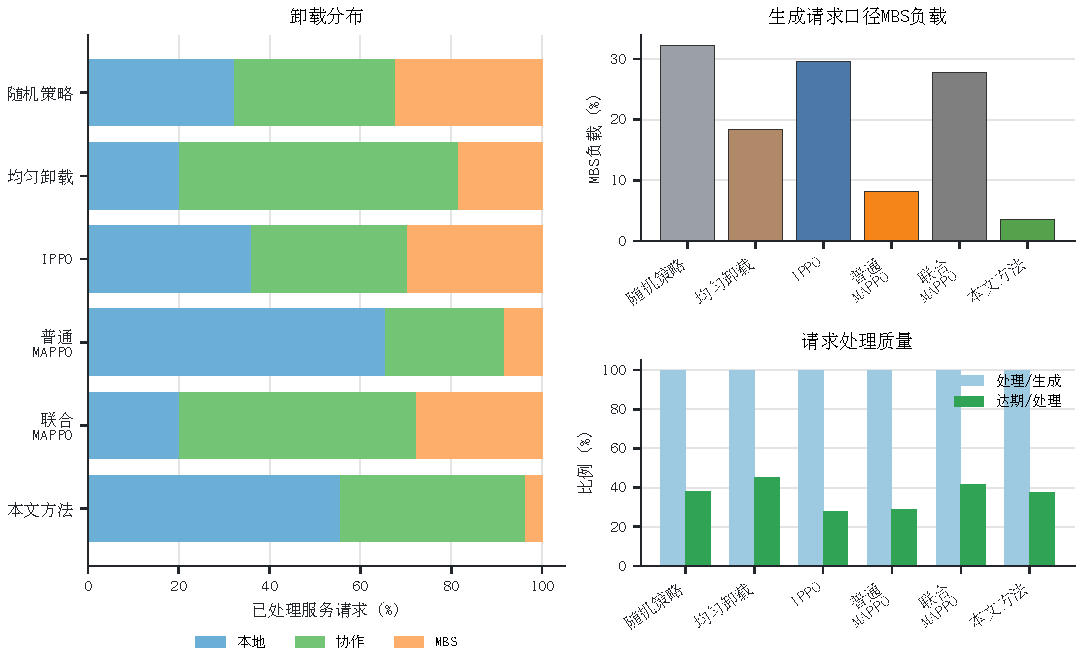
\includegraphics[width=0.94\textwidth]{docs/figures/图5-15_可靠性与卸载机制分析.pdf}
    \bicaption{扩展 baseline 矩阵中的可靠性与卸载机制分析}{Reliability and offloading behavior in the extended baseline matrix}
    \label{fig:baseline-matrix-mechanism}
\end{figure}

图 \ref{fig:baseline-matrix-mechanism} 进一步解释了上述优势的来源。Proposed 的 processed-denominator MBS offloading ratio 为 14.16\%，低于 IPPO 的 18.97\%、Joint MAPPO 的 22.64\% 和 Random 的 30.36\%；generated-denominator MBS load ratio 为 6.63\%，相比 IPPO 和 Random 分别降低约 32.62\% 和 37.06\%。这说明本文方法并非通过简单增加 MBS 依赖来提高服务完成质量，而是在 local、cooperative 和 MBS 之间形成更保守的负载分配。另一方面，Proposed 的 processed request ratio 低于 IPPO 和 Vanilla MAPPO，但 deadline-satisfied-per-processed ratio 分别高出约 22.84\% 和 25.39\%，表明其更倾向于处理更有把握满足 deadline 的请求。综合来看，扩展 baseline 矩阵支持本文方法的核心定位：所提方法追求的是公平、可靠和低 MBS 依赖的多目标折中，而不是在每一个单指标上取得最大值。

\section{参数敏感性与训练收敛分析}
\label{sec:sensitivity}

为进一步验证所提框架的鲁棒性和适用边界，本节从三个维度展开参数敏感性分析：（1）训练完成后系统有效能效的对比；（2）地面节点数量变化下的能效表现；（3）UAV 计算能力变化下的能效表现。

\subsection{有效能效指标定义}
\label{subsec:eee-metric}

为综合衡量系统在能效和服务质量维度的联合表现，本文引入有效能效（Effective Energy Efficiency, EEE）指标：

\begin{equation}
    \text{EEE} = \frac{N_{\text{deadline-satisfied}}}{E_{\text{total}}}
    \label{eq:eee}
\end{equation}

其中 $N_{\text{deadline-satisfied}}$ 为满足截止时间约束的服务请求数，$E_{\text{total}}$ 为 UAV 侧总能耗（单位：Joules）。该指标的物理含义为单位能耗下有效完成的服务请求数，数值越高表示系统在能耗和服务质量之间的权衡越有利。

\subsection{训练收敛分析}
\label{subsec:convergence}

图 \ref{fig:eee-convergence} 给出了 Proposed 与 Vanilla MAPPO 在训练完成（200 episodes）后的 EEE 和 DSR 对比。实验采用 3 个 training seeds（42, 84, 126），在固定 workload seed 42 下评估 6 个 episodes，误差棒表示标准差。

\begin{figure}[!htbp]
    \centering
    
\includegraphics[width=0.88\textwidth]{docs/figures/图5-11_系统有效能效收敛曲线.pdf}
    \bicaption{不同算法训练完成后的有效能效与 DSR 对比}{Effective energy efficiency and DSR comparison after training}
    \label{fig:eee-convergence}
\end{figure}

从图 \ref{fig:eee-convergence} 左图可以看出，Proposed 的 EEE（$0.000108 \pm 0.000025$）略高于 Vanilla MAPPO（$0.000101 \pm 0.000023$），差异约 7\%。右图显示 Proposed 的 DSR（$0.2205 \pm 0.0136$）显著高于 Vanilla MAPPO（$0.1760 \pm 0.0064$），差异约 25\%。这表明双层联合训练在 DSR 维度的改善更为明确，而 EEE 维度的改善幅度较小。需要注意的是，由于缺乏中间 checkpoint 数据，本文无法展示完整的收敛曲线，仅能报告训练完成后的最终对比。

\subsection{地面节点数量敏感性}
\label{subsec:ue-count}

图 \ref{fig:ue-count-sensitivity} 给出了不同地面节点数量（$M = 60, 80, 100, 120, 140$）下三种算法在 energy、latency 和 DSR 三个维度上的表现。实验使用已训练模型（training seeds: 42, 84, 126）在 10 个 workload seeds 下评估，每个 workload seed 运行 6 个 episodes，统计单元为 (training seed, workload seed) 的 episode mean，每个算法每个 UE 数量共 $N=30$ 个样本。误差棒表示跨统计单元的标准差。

\begin{figure}[!htbp]
    \centering
    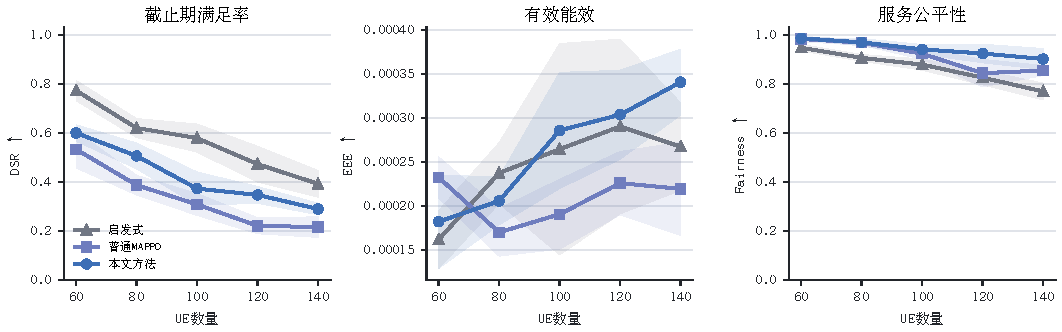
\includegraphics[width=0.96\textwidth]{docs/figures/图5-16_地面节点数量敏感性三指标对比.pdf}
    \bicaption{地面节点数量敏感性三指标对比}{Three-metric sensitivity analysis under different UE counts}
    \label{fig:ue-count-sensitivity}
\end{figure}

从图 \ref{fig:ue-count-sensitivity} 可以看出，随着 UE 数量增加，三种算法的 DSR 均整体下降，说明请求密度升高会加重 UAV-MEC 系统的服务压力。Proposed 在所有 UE 数量下的 DSR 均高于 Vanilla MAPPO，例如在 $M=80$ 时为 0.2591 vs 0.2032，在 $M=120$ 时为 0.1782 vs 0.1505，表明双层分解和注意力建模在不同负载规模下均能改善学习式 baseline 的截止期满足能力。能耗方面，Proposed 在多数 UE 数量下低于 Heuristic，但并不总是低于 Vanilla MAPPO；这与扩展 baseline 矩阵中的结论一致，即本文方法并非单纯追求最低能耗，而是在能耗、服务质量和公平性之间寻求折中。Latency 曲线则显示 Proposed 相对 Heuristic 有明显改善，但在部分 UE 数量下仍高于 Vanilla MAPPO，进一步说明本文方法的主要优势不应表述为最低时延，而应表述为更稳健的多目标服务表现。

\subsection{UAV 算力敏感性}
\label{subsec:uav-cpu}

图 \ref{fig:uav-cpu-sensitivity} 给出了不同 UAV CPU 缩放因子（$0.6\times, 0.8\times, 1.0\times, 1.2\times, 1.4\times$）下三种算法在 energy、latency 和 DSR 上的敏感性表现。基准计算能力范围为 $[40, 90] \times 10^9$ cycles/s。实验设置与地面节点数量敏感性一致（$N=30$）。

\begin{figure}[!htbp]
    \centering
    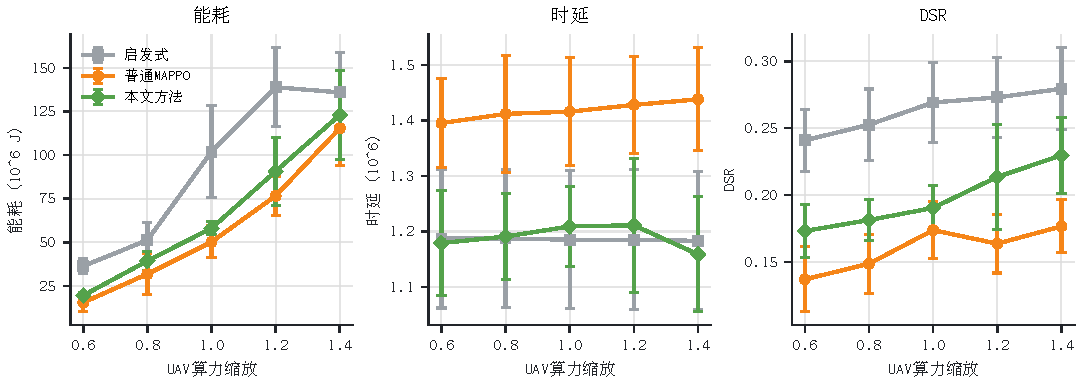
\includegraphics[width=0.96\textwidth]{docs/figures/图5-17_UAV算力敏感性三指标对比.pdf}
    \bicaption{UAV 算力敏感性三指标对比}{Three-metric sensitivity analysis under different UAV computing capacities}
    \label{fig:uav-cpu-sensitivity}
\end{figure}

从图 \ref{fig:uav-cpu-sensitivity} 可以看出，UAV 算力变化会同时影响能耗、时延和 DSR，但三者并不呈简单单调关系。Proposed 在所有算力水平下的 DSR 均高于 Vanilla MAPPO，特别是在 $1.2\times$ 和 $1.4\times$ 时分别达到 0.2135 和 0.2296，而 Vanilla MAPPO 分别为 0.1636 和 0.1766。能耗曲线显示 Proposed 在中等算力区间具有较好的能耗表现，但在低算力和高算力边界处未必优于 Vanilla MAPPO；Latency 曲线同样表明 Proposed 不是所有算力水平下的最低时延方法。该结果说明，固定训练模型在计算资源偏离默认训练分布时会出现适应性边界。总体而言，算力敏感性实验支持本文方法在 DSR 和综合稳定性上的优势，同时也揭示了未来需要进一步研究跨算力分布泛化训练的问题。

\section{DSR-priority 主配置实验}
\label{sec:dsr-priority}

为进一步验证框架在服务质量偏好上的可调节性，本文将 DSR-priority 作为第二组正式主配置进行评估。相较能耗优先配置，DSR-priority 配置将系统级权重调整为 $W_{DSR}=3.0$、$W_E=0.2$；下层 Lagrange 约束目标调整为 $\tau_{dsr}=0.28$、$\tau_{mbs}=0.08$，Lagrange 学习率为 $\eta_{\lambda}=0.5$，乘子上界为 $\lambda_{max}=50.0$；下层 reward 权重调整为 $w_{dead}=7.0$, $w_{succ}=1.5$, $w_{lat}=2.5$, $w_{en}=0.5$, $w_{mbs}=0.2$。

\begin{table}[!htbp]
    \centering
    \bicaption{三种配置下的 Full Hierarchical MARL 对比（$N=30$）}{Full Hierarchical MARL under three configurations ($N=30$)}
    \label{tab:dsr-priority}
    \begin{tabular}{l|rr|rr|rr}
        \hline
        配置 & Reward & & Energy (M) & & DSR & \\
        \hline
        baseline（heuristic） & -5933.9 & & 114.70 & & 0.2734 & \\
        能耗优先（base v2） & -1451.7 & & \textbf{58.06} & & 0.2083 & \\
        DSR 优先（strong） & \textbf{-1147.2} & & 83.04 & & \textbf{0.2435} & \\
        \hline
    \end{tabular}
\end{table}

DSR-priority 配置下，完整方法的 DSR 从能耗优先配置下的 0.2083 提升至 0.2435，与 baseline 的差距从 -0.065 缩小至 -0.030（$p = 1.6\times10^{-6}$）。但该值仍低于 heuristic baseline 的 0.2734，因此本文将其解释为 DSR 的部分恢复，而非完全恢复。DSR-priority 配置下能耗为 83.04M，相比 baseline 的 114.70M 仍节省 27.6\%；cooperative ratio 达到 56.7\%，为所有学习式策略中最高。

\begin{figure}[!htbp]
    \centering
    
\includegraphics[width=0.92\textwidth]{docs/figures/图5-10_DSR优先配置性能权衡.pdf}
    \bicaption{DSR-priority 配置下的性能权衡}{Performance trade-off under the DSR-priority configuration}
    \label{fig:lagrange-tradeoff}
\end{figure}

\begin{figure}[!htbp]
    \centering
    
\includegraphics[width=0.85\textwidth]{docs/figures/fig_hierarchical_training_curves.png}
    \bicaption{固定 workload42 评估曲线}{Fixed workload42 evaluation curves}
    \label{fig:training-curves}
\end{figure}

\section{讨论}
\label{sec:discussion}

\subsection{Energy-DSR-Fairness 三元权衡}
\label{subsec:tradeoff}

实验揭示了多 UAV MEC 系统中一个核心的三元权衡：

\begin{table}[!htbp]
    \centering
    \bicaption{Energy-DSR-Fairness 三元权衡分析}{Energy-DSR-Fairness ternary trade-off analysis}
    \label{tab:tradeoff}
    \begin{tabular}{|l|l|l|}
        \hline
        优化方向 & 优势 & 代价 \\
        \hline
        降低 Energy & 从 114.7M $\rightarrow$ 42.8M (-63\%) & DSR 从 0.27 $\rightarrow$ 0.19 \\
        提升 DSR & 0.27 $\rightarrow$ 0.29 & Energy 维持高位 111.8M \\
        提升 Fairness & 0.77 $\rightarrow$ 0.93 & 依赖更强的轨迹协同建模 \\
        \hline
    \end{tabular}
\end{table}

本文的双层 MARL 框架通过 Lagrange 约束和奖励权重提供了调控这一权衡的机制。第 \ref{sec:dsr-priority} 节的 DSR-priority 主配置实验表明：将 $W_{DSR}$ 从 1.0 提升至 3.0、$W_E$ 从 0.5 降至 0.2、$\tau_{dsr}$ 从 0.18 提升至 0.28 后，完整方法的 DSR 可从 0.2083 部分恢复至 0.2435，与 baseline 的差距缩小约 54\%，同时仍保持约 28\% 的能耗节省。

\subsection{上层轨迹 vs 下层卸载的相对贡献}
\label{subsec:layer-contribution}

对比 \texttt{att+heuristic}（仅上层）和 \texttt{unco+lower}（仅下层）可以分离两层模块的贡献。仅替换上层后，fairness 从 0.775 提升至 0.930，reward 从 -5933.9 提升至 -2128.6，说明轨迹协同主要改善空间覆盖均衡性和系统级奖励。仅替换下层后，energy 从 114.70M 降至 42.85M，但 fairness 基本保持在 0.774 左右，说明卸载学习主要降低能耗并改变执行位置，而不能单独解决空间公平性问题。完整双层方法综合两者，在 reward（-1451.7）、energy（58.06M）和 fairness（0.936）之间形成更均衡的工作点，但 DSR 仍受能耗优先目标限制。

\subsection{与现有工作的对比}
\label{subsec:comparison}

相比黄子祥等 \cite{huang2026madr} 基于 MADRL 的单层端到端方法，本文的双层分解将轨迹控制与请求级卸载拆开处理，降低了直接联合动作建模的结构复杂度，并提高了策略行为的可解释性。相比尤昕阳等 \cite{you2026soft} 的 SAC 方法，本文通过双层拆分分别处理连续轨迹控制与离散请求卸载，减少了直接构造混合联合动作的难度。相比曾耀平等 \cite{zeng2026uav} 的博弈论方法，本文基于 MARL 的在线执行主要依赖局部和邻居观测，具有较好的动态适应性。

\section{本章小结}
\label{sec:summary-chap05}

本章通过固定仿真环境、配对 workload 评估、多组消融实验和扩展 baseline 矩阵验证了所提双层 MARL 框架。实验结果表明，完整双层方法相对基础参考显著提升系统 reward，降低 UAV 侧能耗，提升服务公平性，并将 offline rate 降至 0.00\%。扩展 baseline 矩阵进一步表明，本文方法相对 IPPO、Vanilla MAPPO、Joint MAPPO 和 Random 在 request-weighted DSR、公平性和 MBS 负载控制方面具有明确优势，但并非在 reward、latency、energy 或 DSR 上对所有 baseline 全面最优。上层模块主要贡献在空间部署和公平性，下层模块主要贡献在卸载分布调整和能耗控制；端到端 joint MAPPO 的负向结果进一步说明双层分解具有必要性。本文方法的主要边界在于能耗优先配置会降低 DSR，而 DSR-priority 配置能够将 DSR 从 0.2083 部分恢复至 0.2435，同时仍保持相对 baseline 的能耗节省。
